\documentclass[11pt, oneside]{article}
\usepackage[letterpaper, margin=2cm]{geometry}
\usepackage{AERE546}
\usepackage{xspace}
\newcommand{\xb}{\bar{x}}
\newcommand{\yb}{\bar{y}}

\begin{document}
\noindent \textbf{\Large{Caleb Logemann \\
AER E 546 Fluid Mechanics and Heat Transfer I \\
Homework 6
}}

%\lstinputlisting[language=MATLAB]{H01_23.m}
\begin{enumerate}
  \item % #1
    In order to determine the last boundary condition, we must realize that the
    flow in must be the same as the flow out.
    That is
    \[
      \dintt{0}{1}{\Psi(0, y)}{y} = \dintt{1/4}{1}{\Psi(2, y)}{y}
    \]
    Also in order to be continuous $\Psi(2, 1/4) = 0$ and $\Psi(2, 1) = -1$.
    We can achieve these three conditions with a quadractic polynomial
    $p(y) = ay^2 + by + c$.
    We have the following equations.
    \begin{align*}
      -1 &= a + b + c \\
      0 &= \frac{1}{16} a + \frac{1}{4} b + c \\
      -\frac{1}{2} &= \frac{1}{3}\p{1 - \frac{1}{64}} a + \frac{1}{2}\p{1 - \frac{1}{16}} b + \p{1 - \frac{1}{4}} c
    \end{align*}
    Solving these gives
    \begin{align*}
      a &= \frac{16}{9} \\
      b &= -\frac{32}{9} \\
      c &= \frac{7}{9}
    \end{align*}
    or a boundary condition of
    \[
      \Psi(2, y) = \frac{16}{9}y^2 - \frac{32}{9}y + \frac{7}{9}
    \]

    \lstinputlisting[language=MATLAB]{sor3.m}

    \begin{center}
      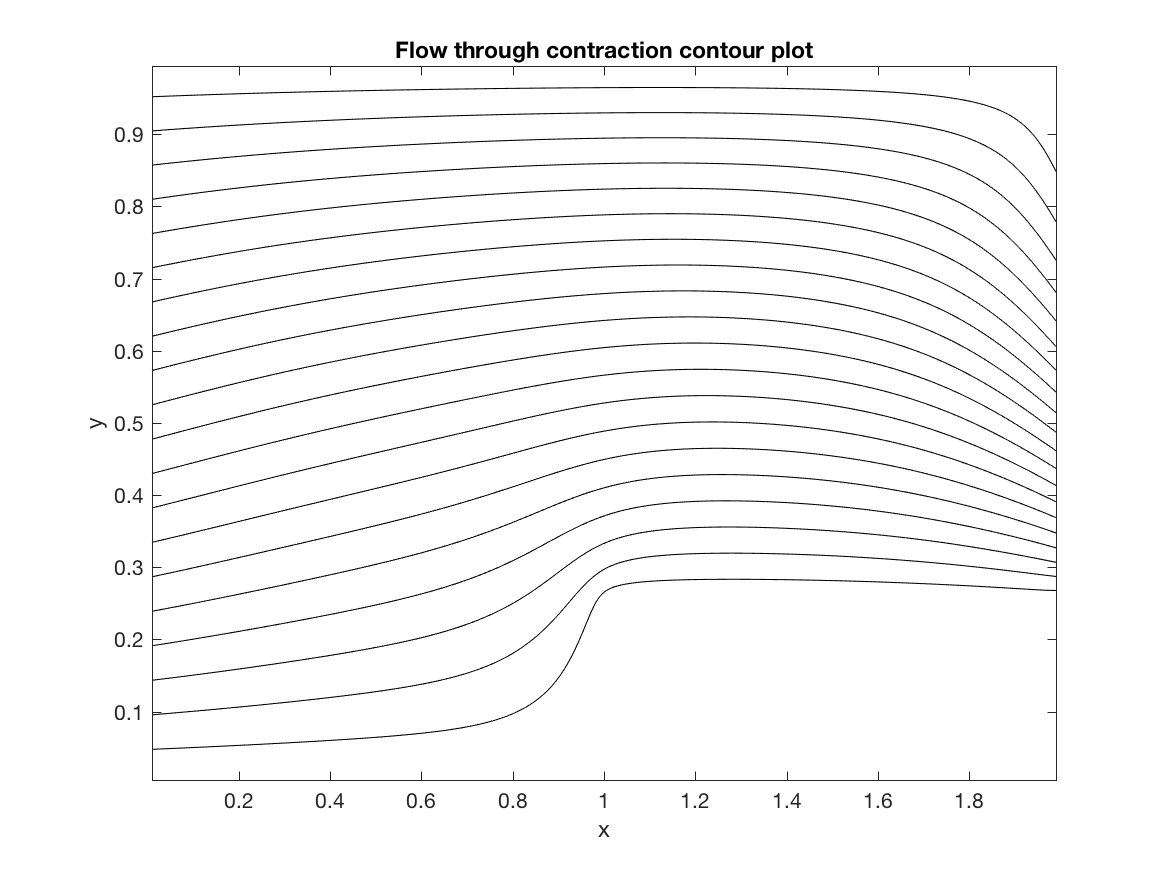
\includegraphics[scale=0.5]{Figures/06_01.png}
      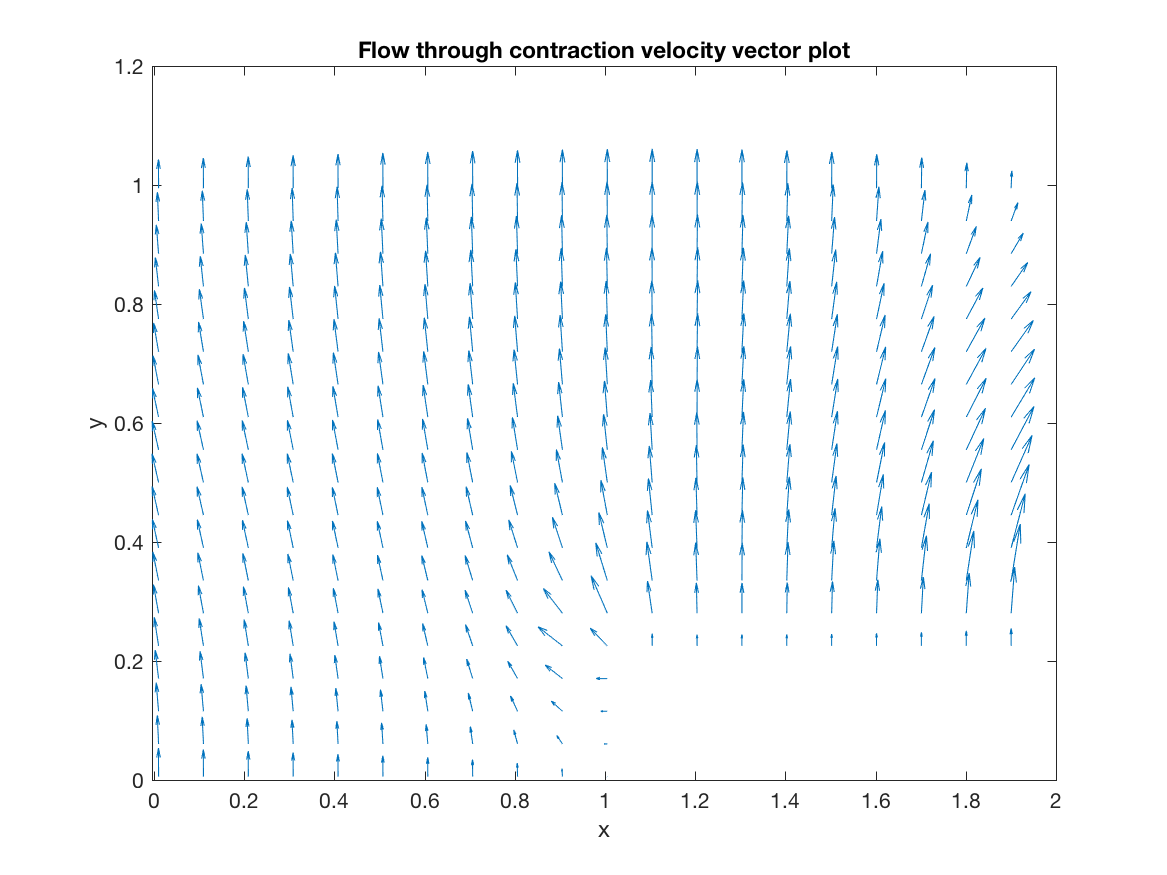
\includegraphics[scale=0.5]{Figures/06_02.png}
    \end{center}

  \item % #2
    The following function runs Gauss-Seidel with SOR on the given problem.
    \lstinputlisting[language=MATLAB]{sor4.m}

    \begin{center}
      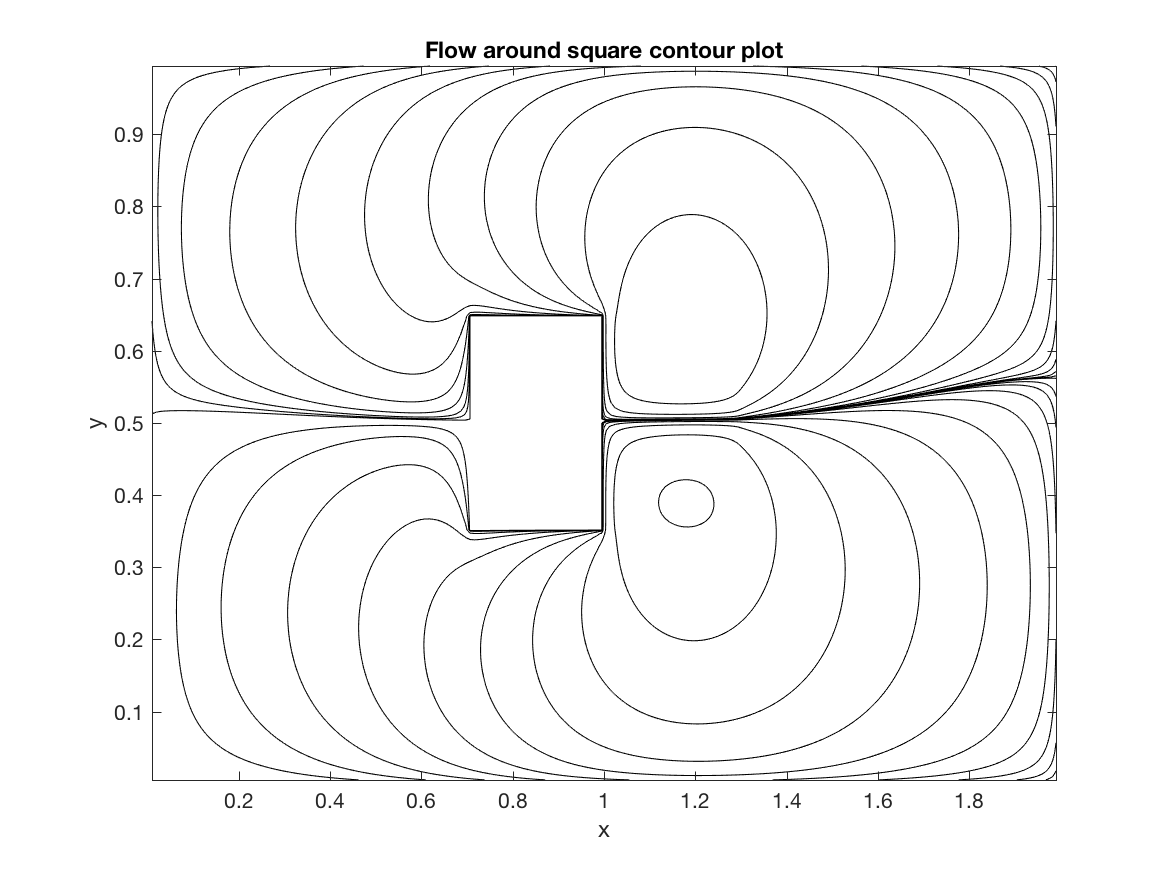
\includegraphics[scale=0.5]{Figures/06_03.png}
      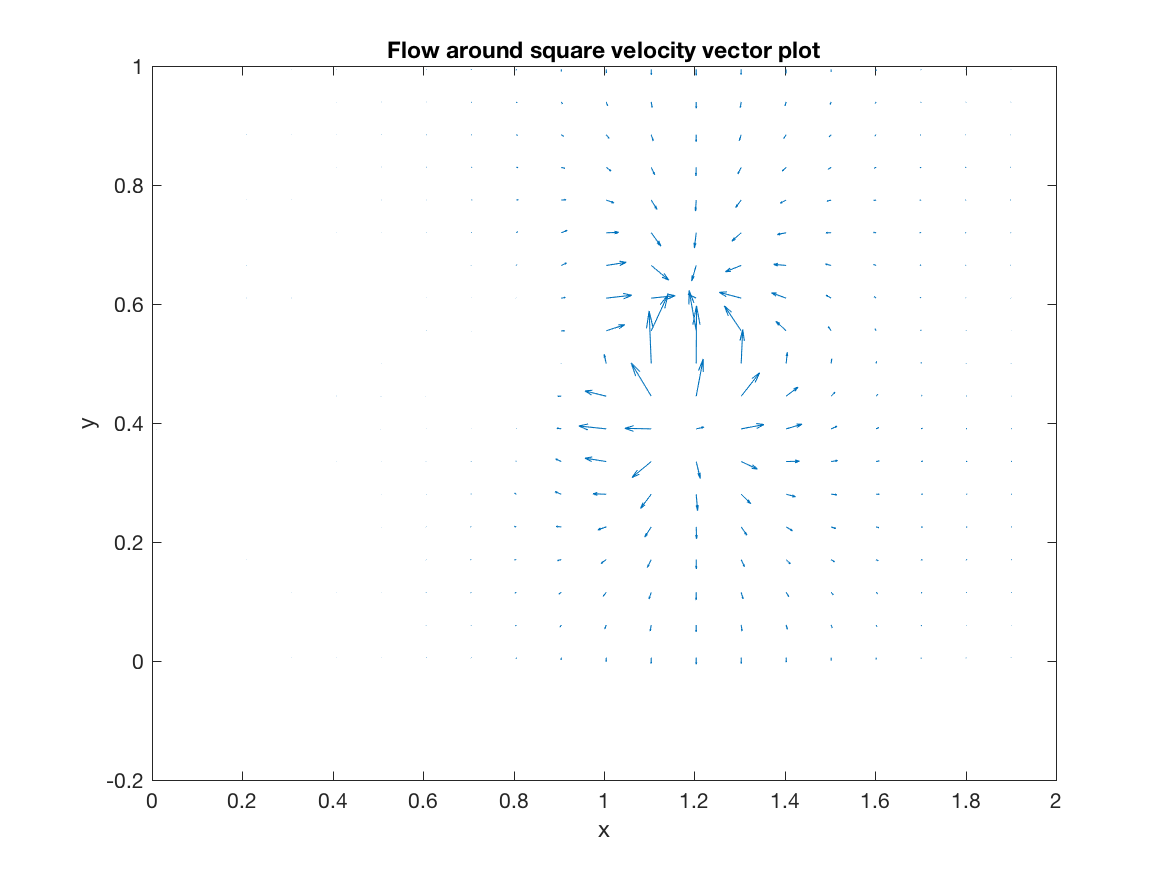
\includegraphics[scale=0.5]{Figures/06_04.png}
    \end{center}


\end{enumerate}
\end{document}
